This chapter explains how we can use the simulator and the pieces we modelled in the preceding chapter to model a whole robot. We then showcase some simulations that were used to validate robot designs and finally present the influence these simulations had on the final design of the robot. 

\section{Overview of the simulation setup}
V-Rep is used to simulate the physics of the robot but the control code runs alongside and not inside V-Rep. This is possible because V-Rep runs a server thread which can process specific instructions\footnote{An alphabetical list of those instructions can be found on \url{http://www.coppeliarobotics.com/helpFiles/en/remoteApiFunctionListAlphabetical.htm}} sent by a client thread. This gives us great implementation flexibility and we can substitute the real robot by the simulation model easily. This is represented on \cref{fig:simulation_principles}.

\begin{figure}[htp]
\center
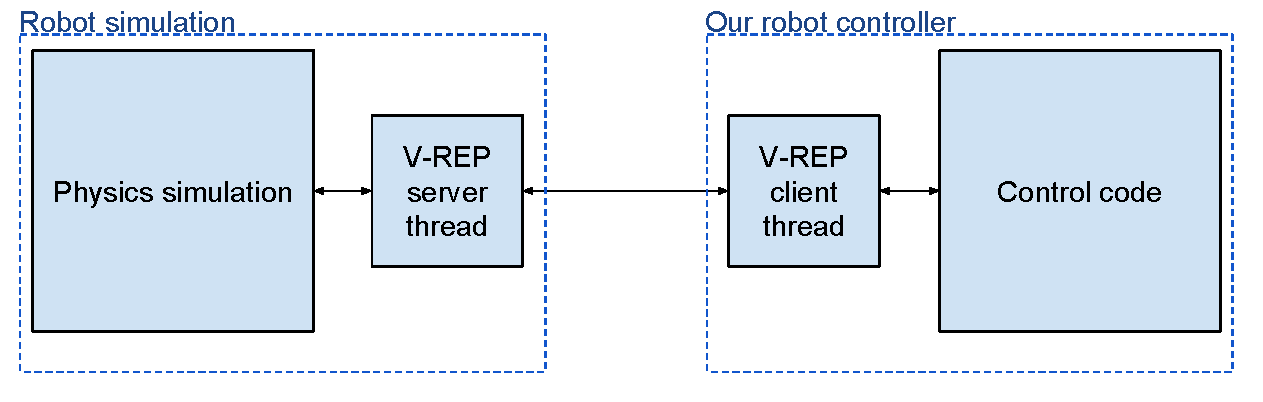
\includegraphics[width=0.6\textwidth]{figures/simulation_principles}
\caption[Simulation principles]{V-Rep simulates the robot while an external program sends order to the robot over TCP/IP thanks to the client/server thread provided by V-Rep.}
\label{fig:simulation_principles}
\end{figure}

Furthermore, the simulation will operate in the synchronous operation mode. That is, each simulation timestep must be triggered by the control code, allowing precise control of the robot. \Cref{fig:remoteApi} presents how V-Rep and the control code interact in synchronous mode.

\begin{figure}[htp]
\center
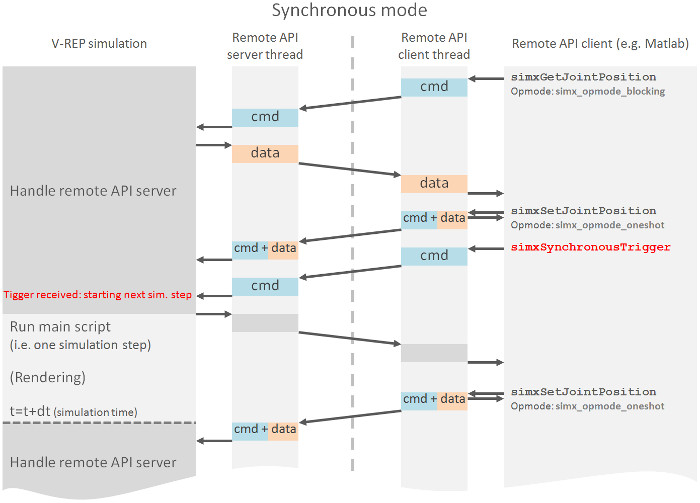
\includegraphics[width=0.6\textwidth]{figures/remoteApiSynchronous}
\caption[Simulation interaction]{Typical interaction between the simulator and the control code. The simulation runs on two threads : the simulation and the server thread. The server threads can receive orders from a client thread which is controlled by a custom application of our own. The simulator waits for a trigger before simulating the next timestep.}
\label{fig:remoteApi}
\end{figure}

The instructions available can execute a number of different actions. The following proved most useful for this project :\begin{itemize}
\item simxGetObjectHandle : this function is used to retrieve a handle on an object. A handle is necessary if a user wants to perform operations on an object.
\item simxSetJointTargetPosition : this function sets a target position for a joint.
\item simxSetFloatSignal : this function gives the possibility of setting the value of a signal inside V-Rep. This is useful if we want to extend the interface that V-Rep provides.
\item simxGetFloatSignal : this function retrieves the value of a float signal. 
\end{itemize}

\lstinputlisting[style=Matlab-editor, float, captionpos=b, caption={Minimal example code that connects to the server, gets the handles and implements a basic control loop}]{codes/simulation_client_vrep.m}

\section{Applications}
\subsection{Static stability}
The first application is simply to build a model of the robot and test if it is able to stand upright on its own, using the servos.

The torque of the servos is computed from the maximal torque of the DC motor and the reduction ratio of the gears. 
\begin{align*}
Torque &= TorqueMotor \times ReductionRatio\\
&= 3.67e^{-3} \times 193\\
&= 0.7083Nm
\end{align*}
In \cref{sec:exp1} we determined that the maximum torque the servo was actually able to produce was $1.7Nm$ so to represent this we choose to set the maximum torque of the servos to $1Nm$.

In V-Rep the different elements of the robot are dynamically enabled and given mass, accordingly to the values listed in \cref{table:weights}. Then, joints (motor controlled with control loop activated) are added to simulate the behaviour of the servos. Their maximal torque is set to $1.6$, the maximum torque developed my Mx-28 servos as shown by our earlier experiments (\cref{table:exp1_results}). 

The springs on the leg are simulated by two spherical joints and one prismatic joint set to spring-damper mode.

The servos of the robot are simply ordered to hold their initial angle and the simulation determines that the robot can indeed stand upright without any active stabilization.

\subsection{Going from a supine to a prone lying position}
The main motivation for a routine that makes the robot move from a supine lying position to a prone one is that it allows us to only have one standing up routine. 

The routine is defined as follows :\begin{enumerate}
\item The robot brings his right arm above his head while preparing the left to lift its body from the left side. The legs are twisted towards the right side.

\item The left left swings towards the right side while the right leg swings towards the left side. The left elbow prepares to push.

\item The left elbow pushes the body up and the hips untwist.

\item When the left leg touches the ground, the robot relaxes all its limb.
\end{enumerate}

\begin{figure}[htp]
\center
    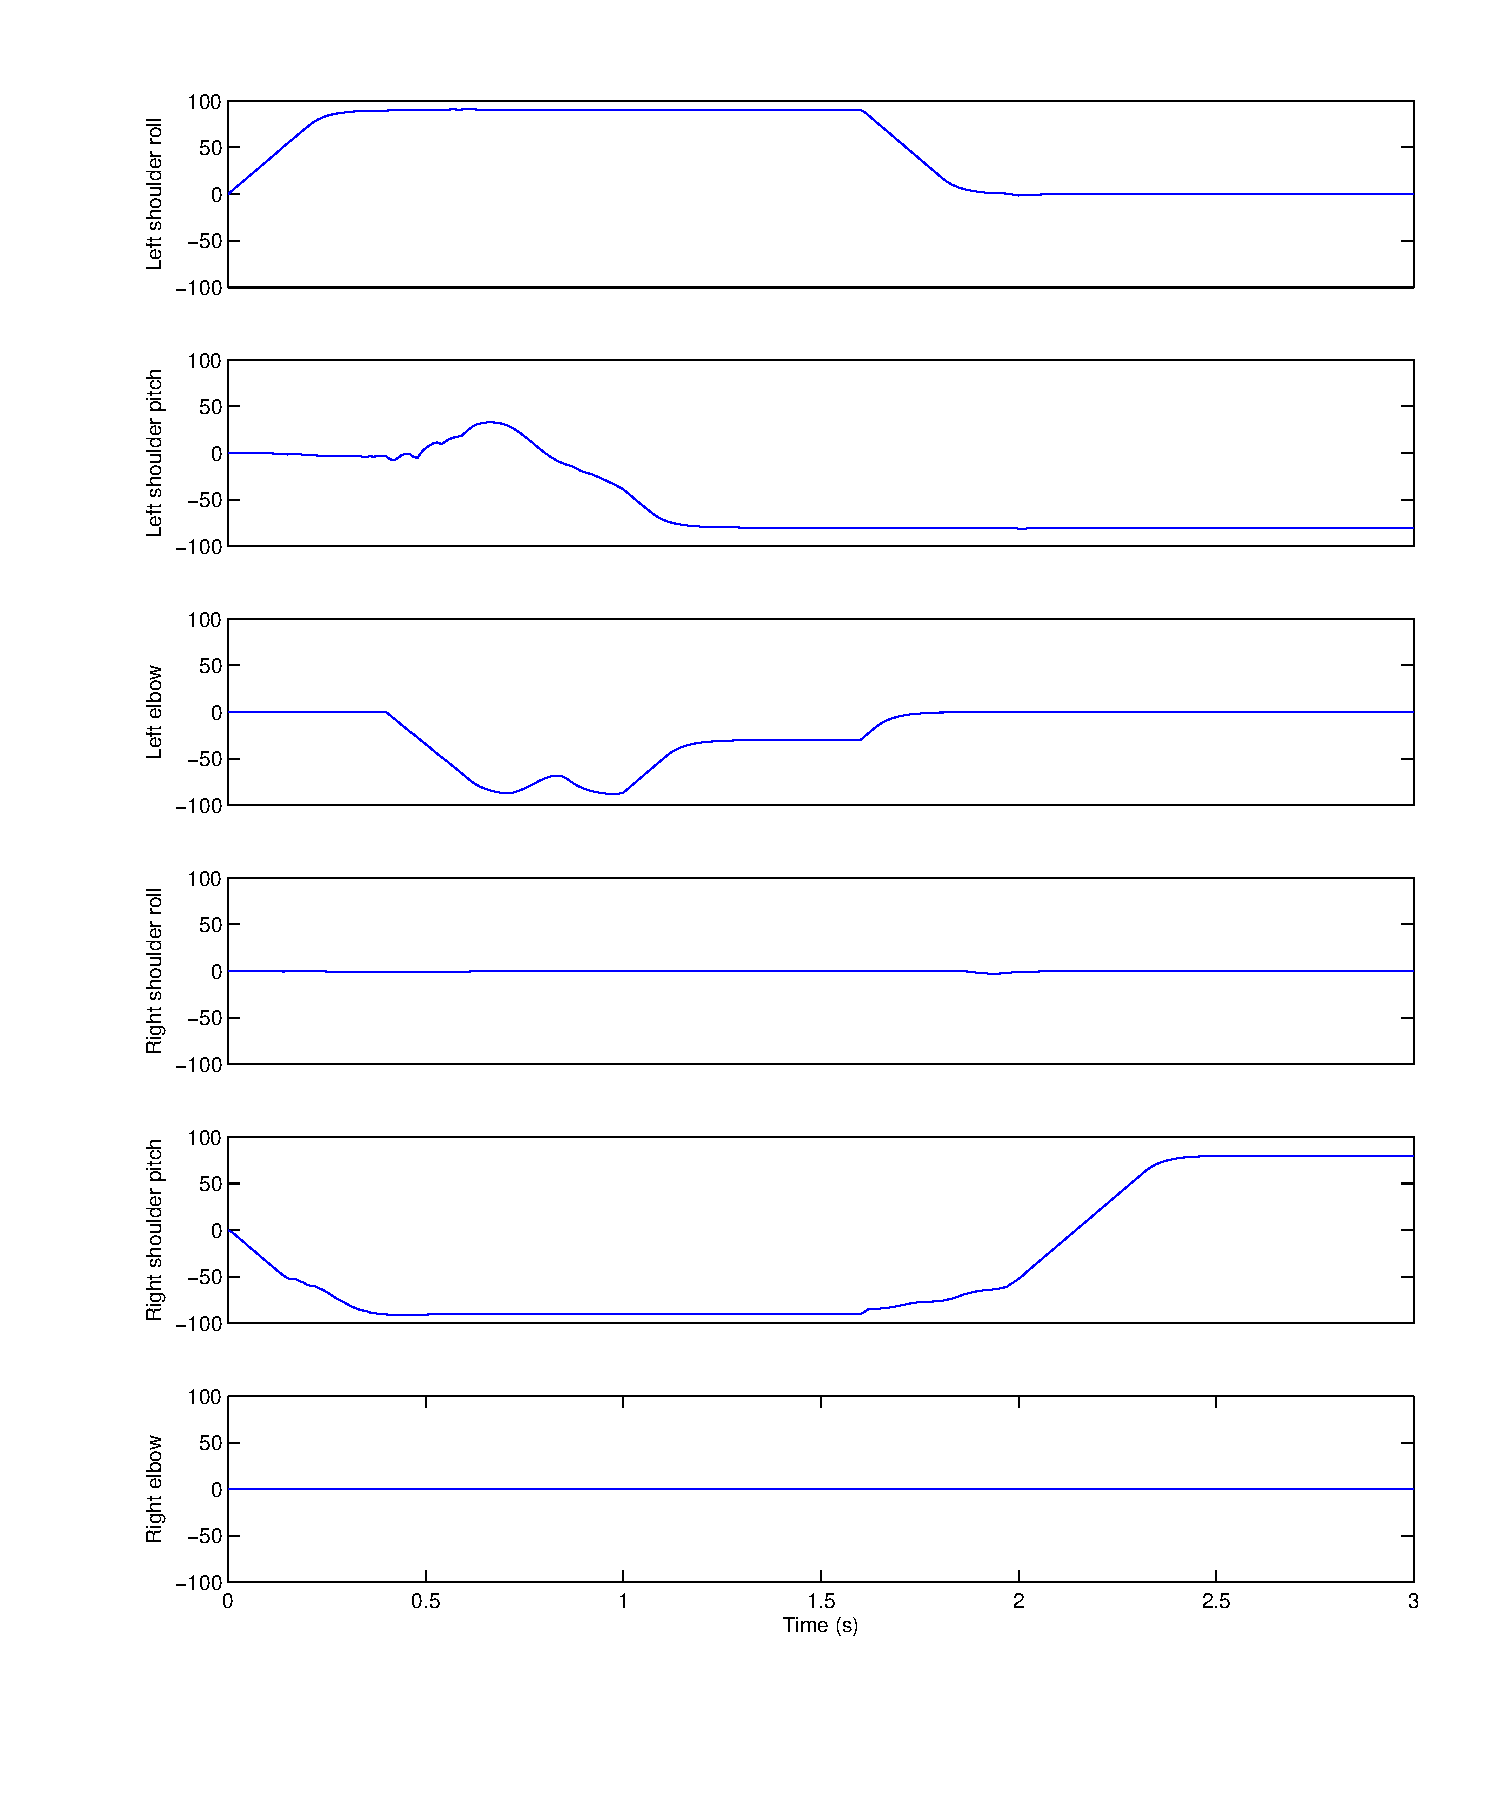
\includegraphics[width = \textwidth]{figures/sup2proneArms}
    \caption[Angles of the arms during \emph{supine} to prone manoeuvre]{Angles of the arms during \emph{supine} to prone manoeuvre}
    \label{fig:sup2proneArms}
\end{figure}

\begin{figure}[htp]
\center
    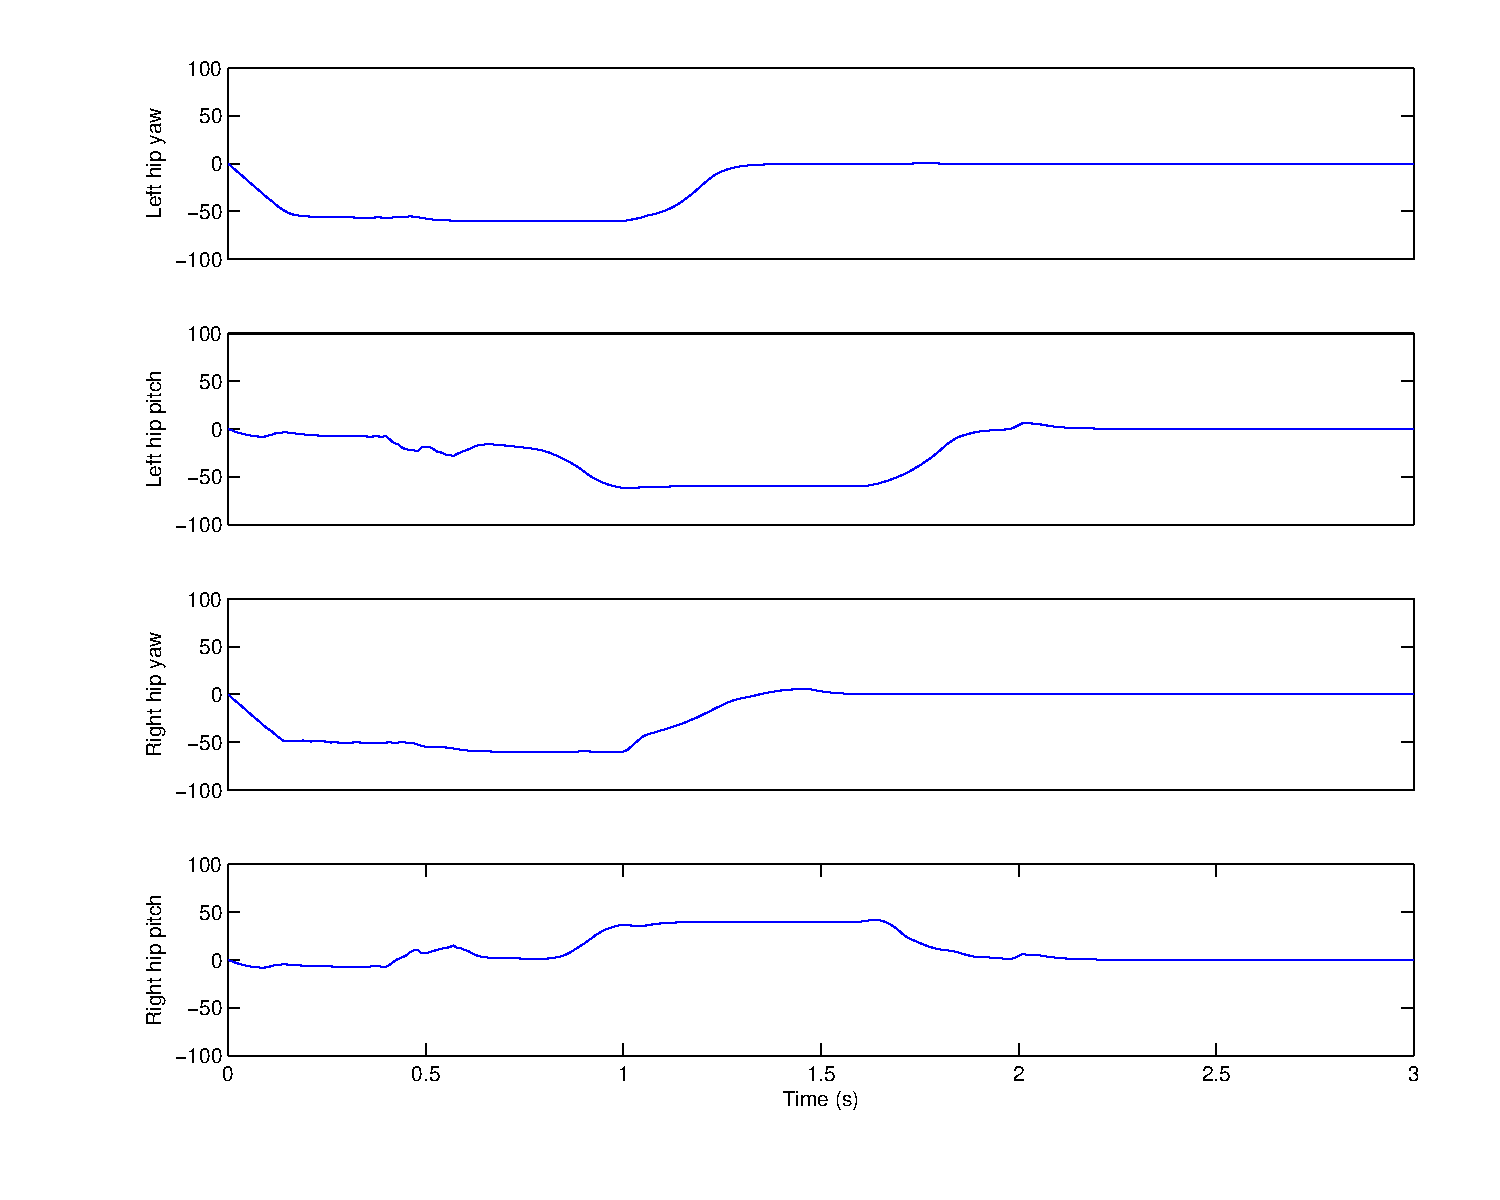
\includegraphics[width = \textwidth]{figures/sup2proneLegs}
    \caption[Angles of the legs during \emph{supine to prone} manoeuvre]{Angles of the legs during \emph{supine to prone} manoeuvre}
    \label{fig:sup2proneLegs}
\end{figure}

\subsection{Standing up from a prone lying position}
This section is heavily inspired by \cite{Stuckler06}

\begin{figure}[htp]
\center
    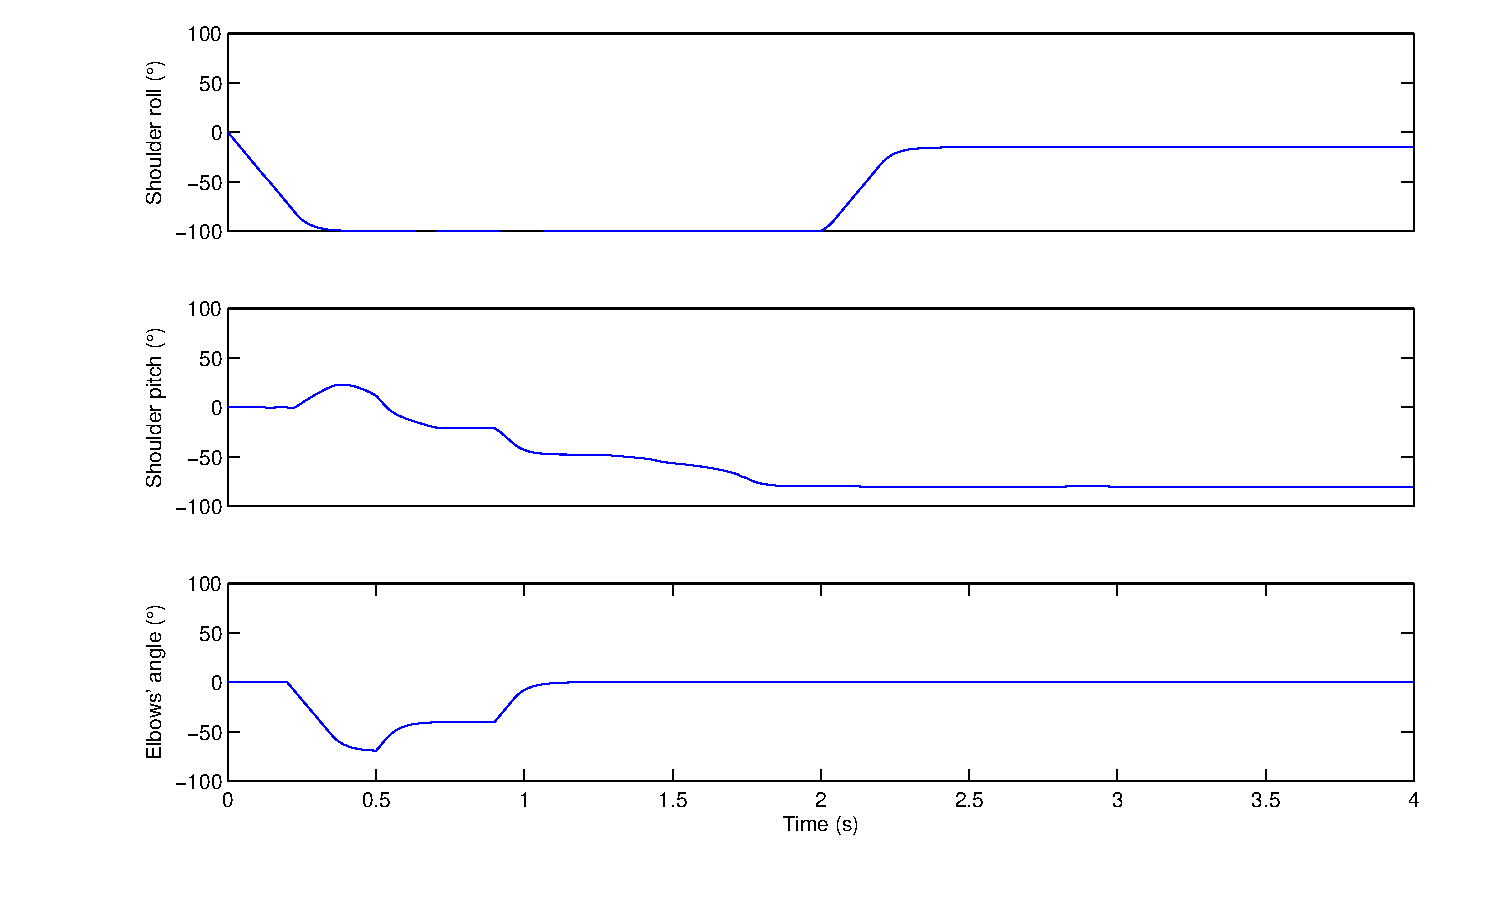
\includegraphics[width = \textwidth]{figures/prone2standArms}
    \caption[Angles of the arms during \emph{supine} to prone manoeuvre]{Angles of the arms during \emph{supine} to prone manoeuvre}
    \label{fig:prone2standArms}
\end{figure}

\begin{figure}[htp]
\center
    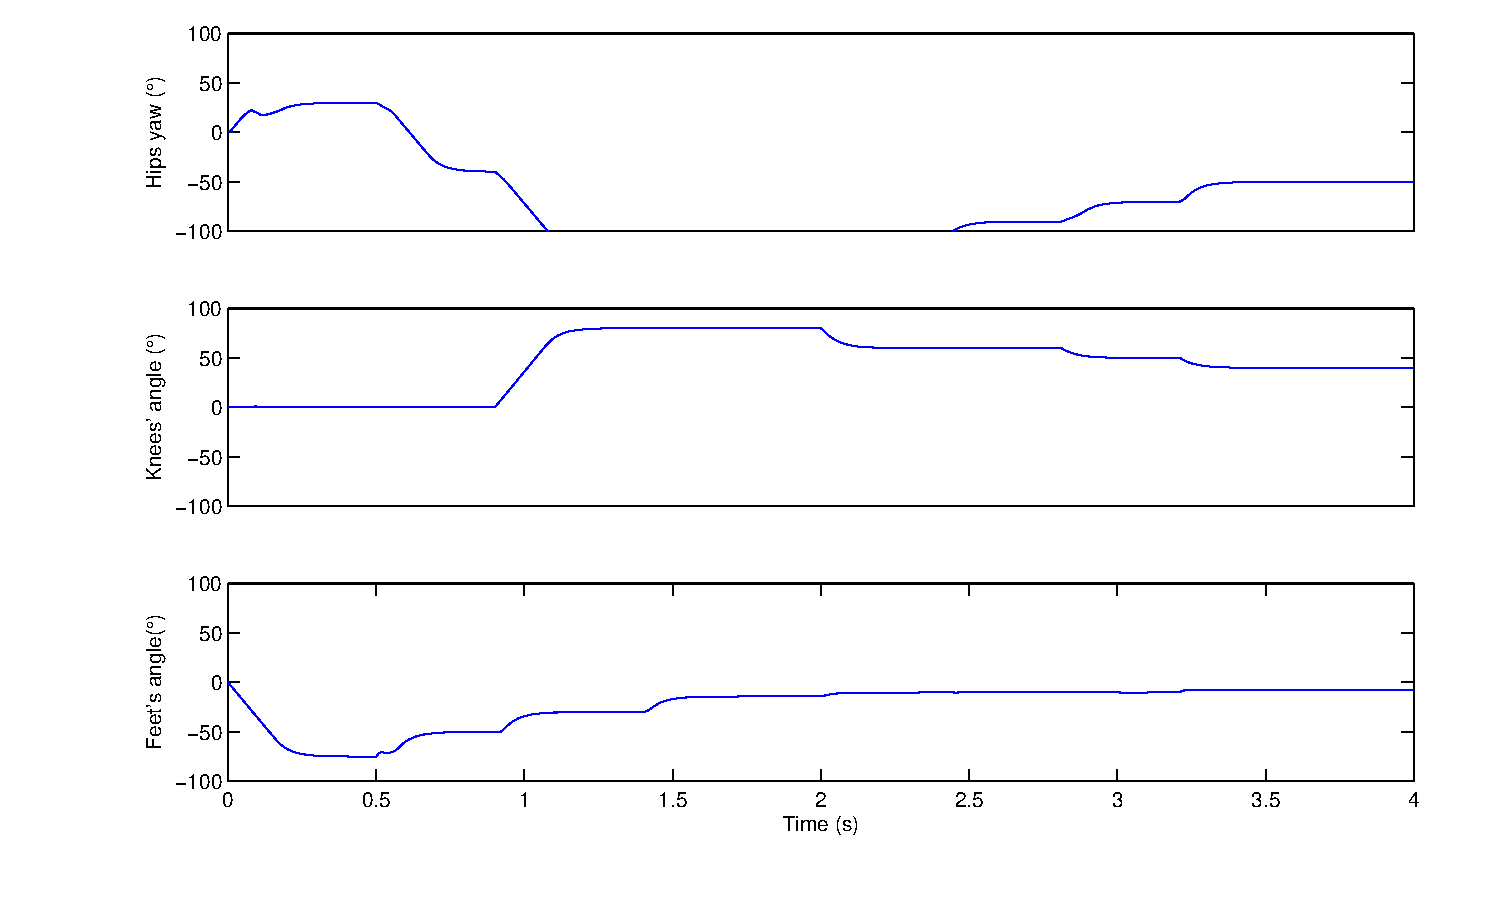
\includegraphics[width = \textwidth]{figures/prone2standLegs}
    \caption[Angles of the legs during \emph{supine to prone} manoeuvre]{Angles of the legs during \emph{supine to prone} manoeuvre}
    \label{fig:prone2standLegs}
\end{figure}

\subsection{Walking}

\section{Influence of the simulations on the final design of the robot}
The simulator helped shape the robot through simulations that unveiled serious design problems (inability to stand after a fall, inability to walk).

The first design is visible on \cref{fig:first_robot}. It was plagued by stability problems, overcomplicated arms and simulation difficulties. 
\begin{figure}[htp]
\center
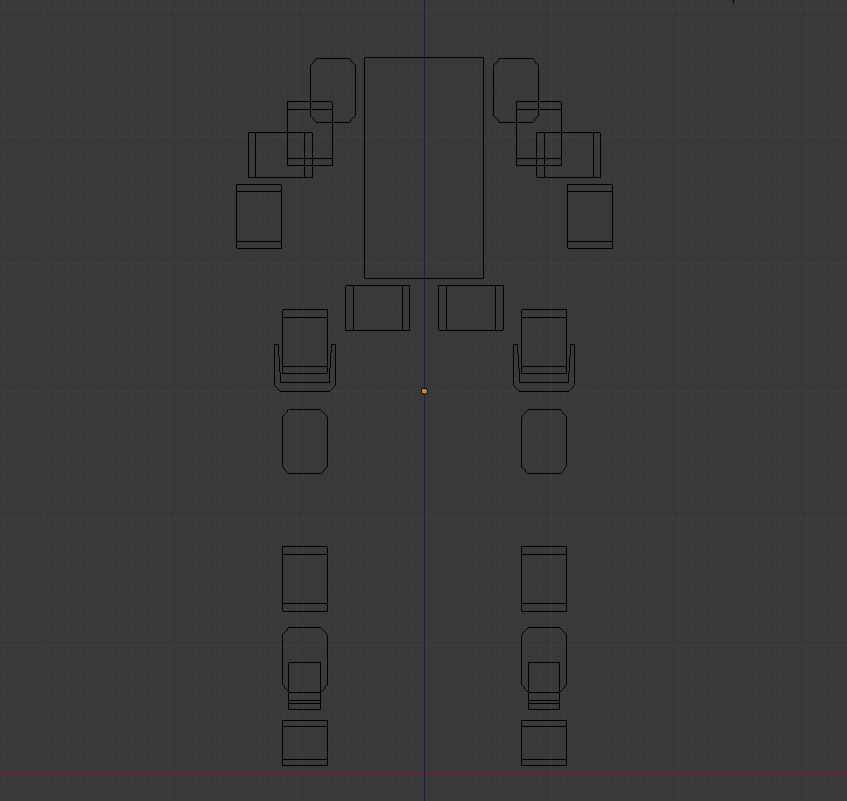
\includegraphics[width=0.6\textwidth]{figures/robot1}
\caption[Initial robot design]{First robot design. Each arm is made of 4 servos, making them quite heavy.}
\label{fig:first_robot}
\end{figure}

The final design, visible on \cref{fig:final_robot} has better stability, wider movement possibilities and can stand up and walk more easily. 
\begin{figure}[htp]
\center
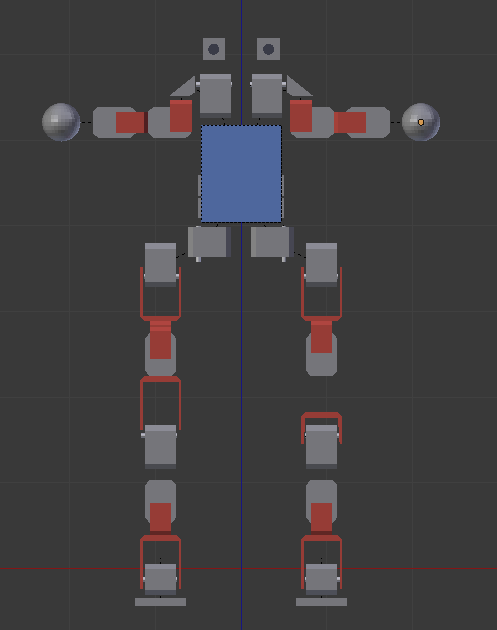
\includegraphics[width=0.6\textwidth]{figures/robot2}
\caption[Final robot design]{Final robot design. Arms now use 3 servos. The feet and the hips use a different configuration to have wider movement possibilities and bring down the center of gravity.}
\label{fig:final_robot}
\end{figure}

The final dimensions of the robot respect the rules of the contest:
\begin{itemize}
\item Height : $61.3cm$
\item Height of COM : $34cm$
\item Height of legs : $cm$
\item Height max is $< 1.5 \times 61.3$.
\item Foot area is $ cm^2$.
\item Weight : $2.726kg$
\end{itemize}